\documentclass[11pt]{article}

\usepackage{verbatim,amsthm,amsmath,amssymb,amsfonts,url}
\usepackage[margin=1in]{geometry}
\usepackage{color}
%Tikz画图
\usepackage{tikz}
\usetikzlibrary{arrows,graphs} %指明是图库

\usepackage[ruled]{algorithm2e}
\usepackage{setspace}

\parindent 0pt
\parskip 3mm

\theoremstyle{definition}
\newtheorem*{solution}{Solution}

% Some useful commands

\newcommand{\CBCMAC}{\text{CBC-MAC}}
\newcommand{\AHMAC}{\mathrm{AHMAC}}
\newcommand{\PHMAC}{\mathrm{PHMAC}}
\renewcommand{\pmod}[1]{\mbox{\ $(\ensuremath{\operatorname{mod}}\ {#1})$}}
\newcommand{\GF}{\mbox{GF}}
\newcommand{\Gl}{\mbox{GL}}


\begin{document}

\begin{center}
{\bf \Large CPSC 413 -- Design and Analysis of Algorithms \uppercase\expandafter{\romannumeral1}

ASSIGNMENT 1}
\end{center}

\hrule 	

\textbf{Name:} Jian Liao

\textbf{Student ID:} 30081230

\textbf{This \LaTeX \ solution template is referenced from CPSC 418 / MATH 318}

\medskip \hrule

\begin{enumerate}

\item[] \textbf{Question 1} ---  For each of the following pairs of functions, $f(n)$ and $g(n)$, indicate whether $f=O(g), f=o(g), f=\Omega(g), f=\omega(g), or f=\Theta(g)$. Give an exhaustive list of all true relationships. No justification required.

\begin{enumerate}
\item %a
$f=2^n, g(n)=n^2$; \\
\textbf{Answer:} $f=\omega(g) \ and\ f=\Omega(g)$ \\

\item %b
$f=2^n, g(n)=2^{2n-4}$; \\
\textbf{Answer:} $f=o(g) \ and\ f=O(g)$ \\		


\item %c
$f(n)=log(n!), g(n)=n^{1.02}$ \\
\textbf{Answer:} $f=\omega(g) \ and\ f=\Omega(g)$ \\

\item %d
$f(n)=n^{cos n}, g(n)=\sqrt{n}$ \\
\textbf{Answer:} The relationship between $f(n)$ and $g(n)$ does not exist. \\

\end{enumerate}

\newpage

\item[] \textbf{Question 2}

\begin{enumerate}

\item %a
Look up the definition of a biconnected undirected graph on Wikipedia. Give a one sentence definition based on induced sub-graphs. Start your definition with “An undirected graph $G=(V, E)$ is biconnected, if ...” \\
\\
\textbf{Answer:} An undirected graph $G=(V, E)$ is biconnected, if $G$ is a connected and "nonseparable" graph, meaning that if any one vertex were to be removed, the graph will remain connected. In other words, a biconnected graph has no articulation vertices.

\item %b
For a directed graph $G=(V, E)$, its underlying undirected graph is obtained by replacing every directed edge $(u, v)$ with an undirected one $\{u, v\}$. (If $(u, v)$ and $(v, u)$ are both in $E$, then the underlying undirected graph still contains only one edge $\{u, v\}$.) \\
\\
Give a strongly connected directed graph such that its underlying undirected graph is not biconnected.
\\\\
\textbf{Answer:} \\

\begin{figure}[htbp]
\centering
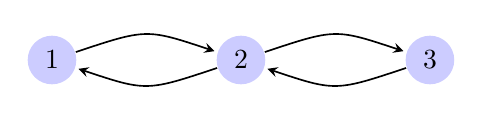
\begin{tikzpicture}[> = stealth, % arrow head style
	shorten > = 1pt, % don't touch arrow head to node
	auto,
	node distance = 3cm, % distance between nodes
	semithick % line style
	,scale=.8,auto=left,every node/.style={circle,fill=blue!20}]
	\node (n1) at (0,0)		{1};
	\node (n2) at (3,0)  	{2};
	\node (n3) at (6,0) 	{3};

	\draw [->] (n1).. controls (1.5,0.5)  ..(n2);
	\draw [->] (n2).. controls (1.5,-0.5)  ..(n1);
	\draw [->] (n2).. controls (4.5,0.5)  ..(n3);
	\draw [->] (n3).. controls (4.5,-0.5)  ..(n2);
\end{tikzpicture}
\caption{\label{fig: } A strongly connected directed graph $G(V, E)$}
\end{figure}

\begin{figure}[htbp]
\centering
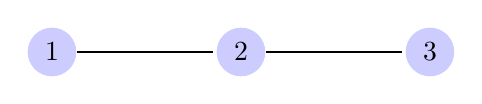
\begin{tikzpicture}[> = stealth, % arrow head style
	shorten > = 1pt, % don't touch arrow head to node
	auto,
	node distance = 3cm, % distance between nodes
	semithick % line style
	,scale=.8,auto=left,every node/.style={circle,fill=blue!20}]
	\node (n1) at (0,0)		{1};
	\node (n2) at (3,0)  	{2};
	\node (n3) at (6,0) 	{3};

	\draw (n1)--(n2);
	\draw (n2)--(n3);

\end{tikzpicture}
\caption{\label{fig: } The underlying undirected graph of $G(V, E)$}
\end{figure}

\textbf{Proof of correctness:} Figure 1 is a strongly connected directed graph because every node $x \in V$, and let $s \in V$, $s$ and $x$ are mutually reachable. Figure 2 is the underlying undirected graph of $G(V, E)$ obtained by replacing every directed edge $(u, v)$ with an undirected one $\{u, v\}$. And Figure 2 is not biconnected because if vertex 2 is removed, the graph will not remain connected, in other words, vertex 2 is an articulation vertex.


\end{enumerate}

\newpage

\item[] \textbf{Question 3} --- Design an algorithm that takes as input a DAG $G = (V, E)$ in adjacency list representation, and outputs for each vertex $v \in V$ the length $d(v)$ of the longest directed path that ends at $v$. For full marks, your algorithm should have worst-case running time $O(|V | + |E|)$. State your algorithm’s worst-case running time, and provide a brief justification for correctness and for your running time statement.

\textbf{Answer:}

\begin{algorithm}[H]
\caption{The longest directed path in a DAG}%算法名字
\LinesNumbered %要求显示行号
% and a source vertex s
\KwIn{A DAG $G=(V,E)$ in adjacency list representation}%输入参数
\KwOut{For each vertex $v \in V$ the length $d(v)$ of the longest directed path that ends at $v$}%输出
Run \textbf{topological sort} on the input DAG $G=(V,E)$, return a topological order of $G$ and store it in a \textbf{Stack}\; %\;用于换行

$int\ dist[V]$\;

\For{$i=0 \to V$}{
  $dist[i] \gets 0$; \tcp{\color{blue}Initialize distances to all vertices as 0}
}
% $dist[s] \gets 0$; \tcp{\color{blue}Set distance to source as 0}
% \tcc{\color{blue}Set source vertex to the first vertex that satisfies $InDegrees=0$}
% $int\ source \gets Stack.top()$\; 
% $dist[source] \gets 0$; \tcp{\color{blue}Set distance to source vertex as 0}
\tcp{\color{blue}Process vertices in topological order}
\While{Stack is not empty}{
  \tcp{\color{blue}Get the next vertex from topological order}
  $int\ u \gets Stack.pop()$\;
  % \If{$dist[u] \neq INF$ and Stack is not empty}{
  % 	$int\ v \gets Stack.top()$; \tcp{\color{blue}Get the next vertex in topological order}
  %   $dist[v] \gets dist[u]+1$; \tcp{\color{blue}Set dist[nextVertex] to dist[preVertex] + 1}
  % }
  \tcp{\color{blue}Update distances of all adjacent vertices}
  \ForEach{$v \in Adj[u]$}{
  	$dist[v] \gets max(d[v],d[u]+1)$\;
  }

}

\For{$i=0 \to V$}{
	\tcp{\color{blue}Return the $d(v)$ of the longest directed path that ends at each vertex}
	\Return{dist[i]}\; 
}

\end{algorithm}

% And also the longest path from source vertex $V_S$ to vertex $V_N$ is by following the linear topological order which is $|V_S \to V_N|$.
% In this linear order, it shows that it cannot reach to vertex $V_1$ from the source vertex $V_S$. Also, suppose there exists an edge $(V_S, V_N)$, which means there is a direct path from $V_S$ to $V_N$, the distance between $V_S$ and $V_N$ will be 1. And obviously it shortens the distance between $V_S$ and $V_N$ if there is any connected path from $V_S$ to $V_N$ besides the linear topological order. By induction, the longest path from $V_S$ to $V_N$, where $V_N$ appears after the $V_S$ in the linear topological order of $G$, is by following the linear topological order which is $|V_S \to V_N|$. In this algorithm, the special case is that the source vertex is the first vertex that satisfies $InDegrees=0$ in the topological order. Thus, the longest path ($d(v)$) from $V_S$ to each vertex $v \in V$ is $|V_S \to V_v|$.

\textbf{Proof of analysis:} Time complexity of topological sorting is $O(|V|+|E|)$. After sorting this graph $G$, the algorithm processes all adjacent vertices for every vertex, it runs a loop for all adjacent vertices. Total adjacent vertices in a graph is $O(|E|)$. So the inner loop runs $O(|V|+|E|)$ times. And also the algorithm will print the results which is $O(|V|)$. Therefore, overall time complexity of this algorithm is $O(|V|+|E|+|V|+|E|+|V|)$, which is $O(|V|+|E|)$.\\
\\
\textbf{Proof of correctness:} For every DAG $G=(V, E)$, there must exist a topological order representing a linear order $(V_S, ..., V_N)$ of this graph $G$. In this algorithm, it initializes the distances to all vertices as 0 and then finds out the topological order of this graph $G$. Then the algorithm processes all vertices one by one in topological order. For every vertex being processed, the algorithm updates distances of its adjacent vertices using the distance of current vertex which is $d[u]+1$, or the distances remain the same if $d[v] \ge d[u]+1$. After the algorithm processing all the vertices one by one in topological order, the distance $dist[v]$ of each vertex $v \in V$ is the longest directed path that ends at $v$ in $G$. \\\\ This can be proved by induction. The base case is that $G(V_1,...,V_N, E)$ only has the edges \{$(V_1,V_2), (V_2,V_3),...,(V_{N-1},V_N)$\}, the topological order of $G$ is exactly $(V_1,...,V_N)$ and the distance of the longest directed path of each vertex $v \in V$ is exactly the distance of $|V_1 \to V_v|$. 

\begin{figure}[htbp]
\centering
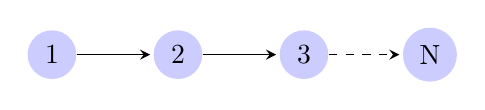
\begin{tikzpicture}[> = stealth, % arrow head style
	shorten > = 1pt, % don't touch arrow head to node
	auto,
	node distance = 3cm, % distance between nodes
	semithick % line style
	,scale=.8,auto=left,every node/.style={circle,fill=blue!20}]
	\node (n1) at (0,0)		{1};
	\node (n2) at (2,0)  	{2};
	\node (n3) at (4,0)  	{3};
	\node (nN) at (6,0) 	{N};

	\draw[->] (n1)--(n2);
	\draw[->] (n2)--(n3);
	\draw[->,dashed] (n3)--(nN);

\end{tikzpicture}
\caption{\label{fig: } The base case of $G(V_1,...,V_N, E)$}
\end{figure}
Assume adding an edge $(V_1,V_N)$ to $G$, the distance of the longest direted path that ends at vertex $N$ still remain the same as $|V_1 \to V_N|$. Because when the algorithm is processing $V_1$, $V_N$ is one of its adjacent vertices, then $dist[V_N]$ will be set to $dist[V_1]+1=1$. After N-1 steps, the algorithm will process $V_{N-1}$ and update $dist[V_N]$ to $dist[V_{N-1}]+1$, which is still $|V_1 \to V_N|$ eventually. By induction, adding any edges $(V_x,V_y), (V_x, V_y \in V)$ to $E$ in topological order will not be changing the distance of the longest directed path that ends at each vertex.
\begin{figure}[htbp]
\centering
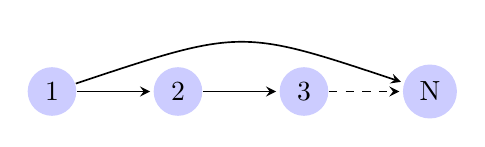
\begin{tikzpicture}[> = stealth, % arrow head style
	shorten > = 1pt, % don't touch arrow head to node
	auto,
	node distance = 3cm, % distance between nodes
	semithick % line style
	,scale=.8,auto=left,every node/.style={circle,fill=blue!20}]
	\node (n1) at (0,0)		{1};
	\node (n2) at (2,0)  	{2};
	\node (n3) at (4,0)  	{3};
	\node (nN) at (6,0) 	{N};

	\draw[->] (n1)--(n2);
	\draw[->] (n2)--(n3);
	\draw[->,dashed] (n3)--(nN);
	\draw[->] (n1).. controls (3,1)  ..(nN);

\end{tikzpicture}
\caption{\label{fig: } Adding an edge $(V_1,V_N)$ to $G(V_1,...,V_N, E)$}
\end{figure}

Assume adding a vertex $V_M$ that also satisfies $InDegrees=0$ and an edge $(V_M,V_N)$ to the graph in topological order, the distance of the longest direted path that ends at vertex $N$ still remain the same as $|V_1 \to V_N|$, and also it satisfies $dist[V_M]=0$. Because when the algorithm is processing $V_M$, $V_N$ is its adjacent vertex, then $dist[V_N]$ will be set to $dist[V_M]+1=1$ and $dist[V_M]$ remains 0. After N-1 steps, the $dist[V_N]$ will be updated to $dist[V_{N-1}]+1$, which is still $|V_1 \to V_N|$ eventually. By induction, adding any vertices $V_v$ that satisfies $InDegress=0$ and edges $(V_v,V_n), (V_v, V_n \in V)$ to $E$ in topological order will not be changing the distance of the longest directed path that ends at each vertex.

\begin{figure}[htbp]
\centering
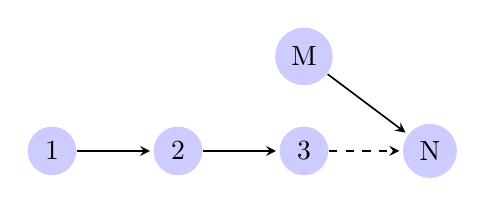
\begin{tikzpicture}[> = stealth, % arrow head style
	shorten > = 1pt, % don't touch arrow head to node
	auto,
	node distance = 3cm, % distance between nodes
	semithick % line style
	,scale=.8,auto=left,every node/.style={circle,fill=blue!20}]
	\node (n1) at (0,0)		{1};
	\node (n2) at (2,0)  	{2};
	\node (n3) at (4,0)  	{3};
	\node (nM) at (4,1.5)  	{M};
	\node (nN) at (6,0) 	{N};

	\draw[->] (n1)--(n2);
	\draw[->] (n2)--(n3);
	\draw[->,dashed] (n3)--(nN);
	\draw[->] (nM)--(nN);

\end{tikzpicture}
\caption{\label{fig: } Adding a vertex $V_M$ and an edge $(V_M,V_N)$ to $G(V_1,...,V_N, E)$}
\end{figure}

Proved by induction as required. After the algorithm processing all the vertices one by one in topological order, the distance $dist[v]$ of each vertex $v \in V$ is the longest directed path that ends at $v$ in $G$.


\newpage

\item[] \textbf{Question 4} --- Design an algorithm that outputs for a given list of n integers, one of the integers that occurs most often in the list. E.g., if the list is (1, 5, 3, 5, 1, 2, 7, 5, 3, 4, 9, 3), then the algorithm might output either 3 or 5, because both integers occur three times in the list, while every other integer occurs only once or twice. For full marks your algorithm should have worst-case running time $O(n log n)$. State your algorithm’s worst-case running time, and provide a brief justification for correctness and for your running time statement.

\textbf{Answer:}

\begin{algorithm}[H]
\caption{Find integer(s) that occurs most often in the list}%算法名字
\LinesNumbered %要求显示行号
\KwIn{A list of integers}%输入参数
\KwOut{The integer(s) that occurs most often in the list}%输出
Run \textbf{merge sort} on the input list of integers in descending order, return a sorted list of integers \textbf{List}\; %\;用于换行

$int\ max$; \tcp{\color{blue}Temporary num}
$int\ count \gets 1$; \tcp{\color{blue}Temporary count}
$int\ maxcount \gets count$; \tcp{\color{blue}Store the max count}
$int\ maxnum$; \tcp{\color{blue}Store the max num}

\For{$i=0 \to List.size-1$}{
  $max \gets List[i]$\;
  \eIf{List[i+1]==max}
  {$count++$\;}{$count \gets 1$\;}
  \tcp{\color{blue}FindMax}
  \If{$count > maxcount$}{
  $maxcount \gets count$; \tcp{\color{blue}Store the maxcount}
  $maxnum \gets max$; \tcp{\color{blue}Store the maxnum}

  }
}
\Return{maxnum\;}
\end{algorithm}

\textbf{Proof of analysis:} Time complexity of merge sort is $O(nlogn)$. After sorting the input list of integers. The algorithm processes all the elements in the list, which is $O(n)$. Therefore, overall time complexity of this algorithm is $O(nlogn+n)$, which is $O(nlogn)$.\\
\\
\textbf{Proof of correctness:} By sorting the list, the integers that are the same will be placed together and sorted in descending order. Therefore, the algorithm can easily count the occurence of each interger in the list by doing a traversal of the list. And essentially, the algorithm will find the max count and also the integer that occurs most often in the list, which is similar to the process of FindMax.

\end{enumerate}

\newpage

\begin{center}
\textbf{{\LARGE Cover Page for CPSC 413 \\Homework Assignment \#1}}
\end{center}

\textbf{Name:} \underline{\hbox to 145mm{\leftline {Jian Liao}}}
\\\\
\textbf{Course Section:} \underline{\hbox to 127mm{\leftline {CPSC 413 Tutorial 01}}}
\\

\textbf{Collaborators:}
\\\\
Question1: \underline{\hbox to 140mm{\leftline {N/A}}}
\\\\
Question2: \underline{\hbox to 140mm{\leftline {N/A}}}
\\\\
Question3: \underline{\hbox to 140mm{\leftline {N/A}}}
\\\\
Question4: \underline{\hbox to 140mm{\leftline {N/A}}}
\\

\textbf{Other Sources:}
\\\\
Question1: \underline{\hbox to 140mm{\leftline {N/A}}}
\\\\
Question2: \underline{\hbox to 140mm{\leftline {https://en.wikipedia.org/wiki/Biconnected\_graph}}}
\\\\
Question3: \underline{\hbox to 140mm{\leftline {https://www.geeksforgeeks.org/shortest-path-for-directed-acyclic-graphs/}}}
\\\\
Question4: \underline{\hbox to 140mm{\leftline {https://blog.csdn.net/Allenalex/article/details/10830797}}}
\\

\textbf{Declaration:}
\\\\
{\small I have written this assignment myself. I have not copied or used the notes of any other student.}
\\\\
\textbf{Date/Signature:} \underline{\hbox to 127mm{\leftline {Jian Liao, May 23, 2019}}}

\end{document}
